\documentclass[10pt,a4paper,onecolumn]{article}
\usepackage{marginnote}
\usepackage{graphicx}
\usepackage{xcolor}
\usepackage{authblk,etoolbox}
\usepackage{titlesec}
\usepackage{calc}
\usepackage{tikz}
\usepackage{hyperref}
\hypersetup{colorlinks,breaklinks,
            urlcolor=[rgb]{0.0, 0.5, 1.0},
            linkcolor=[rgb]{0.0, 0.5, 1.0}}
\usepackage{caption}
\usepackage{tcolorbox}
\usepackage{amssymb,amsmath}
\usepackage{ifxetex,ifluatex}
\usepackage{seqsplit}
\usepackage{fixltx2e} % provides \textsubscript
\usepackage[
  backend=biber,
%  style=alphabetic,
%  citestyle=numeric
]{biblatex}
\bibliography{mybibfile.bib}



% --- Page layout -------------------------------------------------------------
\usepackage[top=3.5cm, bottom=3cm, right=1.5cm, left=1.0cm,
            headheight=2.2cm, reversemp, includemp, marginparwidth=4.5cm]{geometry}

% --- Default font ------------------------------------------------------------
% \renewcommand\familydefault{\sfdefault}

% --- Style -------------------------------------------------------------------
\renewcommand{\bibfont}{\small \sffamily}
\renewcommand{\captionfont}{\small\sffamily}
\renewcommand{\captionlabelfont}{\bfseries}

% --- Section/SubSection/SubSubSection ----------------------------------------
\titleformat{\section}
  {\normalfont\sffamily\Large\bfseries}
  {}{0pt}{}
\titleformat{\subsection}
  {\normalfont\sffamily\large\bfseries}
  {}{0pt}{}
\titleformat{\subsubsection}
  {\normalfont\sffamily\bfseries}
  {}{0pt}{}
\titleformat*{\paragraph}
  {\sffamily\normalsize}


% --- Header / Footer ---------------------------------------------------------
\usepackage{fancyhdr}
\pagestyle{fancy}
\fancyhf{}
%\renewcommand{\headrulewidth}{0.50pt}
\renewcommand{\headrulewidth}{0pt}
\fancyhead[L]{\hspace{-0.75cm}\includegraphics[width=5.5cm]{C:/Users/sibarrae/AppData/Local/Programs/R/R-4.4.2/library/rticles/rmarkdown/templates/joss/resources/JOSS-logo.png}}
\fancyhead[C]{}
\fancyhead[R]{}
\renewcommand{\footrulewidth}{0.25pt}

\fancyfoot[L]{\footnotesize{\sffamily Ibarra-Espinosa and Hu, (2024). R
Tools for ObsPack, Receptors and Footprints (rtorf) for processing
atmospheric observations in NOAA-GML '
ObsPack. \textit{Journal of Open Source Software}, (), . \href{https://doi.org/}{https://doi.org/}}}


\fancyfoot[R]{\sffamily \thepage}
\makeatletter
\let\ps@plain\ps@fancy
\fancyheadoffset[L]{4.5cm}
\fancyfootoffset[L]{4.5cm}

% --- Macros ---------

\definecolor{linky}{rgb}{0.0, 0.5, 1.0}

\newtcolorbox{repobox}
   {colback=red, colframe=red!75!black,
     boxrule=0.5pt, arc=2pt, left=6pt, right=6pt, top=3pt, bottom=3pt}

\newcommand{\ExternalLink}{%
   \tikz[x=1.2ex, y=1.2ex, baseline=-0.05ex]{%
       \begin{scope}[x=1ex, y=1ex]
           \clip (-0.1,-0.1)
               --++ (-0, 1.2)
               --++ (0.6, 0)
               --++ (0, -0.6)
               --++ (0.6, 0)
               --++ (0, -1);
           \path[draw,
               line width = 0.5,
               rounded corners=0.5]
               (0,0) rectangle (1,1);
       \end{scope}
       \path[draw, line width = 0.5] (0.5, 0.5)
           -- (1, 1);
       \path[draw, line width = 0.5] (0.6, 1)
           -- (1, 1) -- (1, 0.6);
       }
   }

% --- Title / Authors ---------------------------------------------------------
% patch \maketitle so that it doesn't center
\patchcmd{\@maketitle}{center}{flushleft}{}{}
\patchcmd{\@maketitle}{center}{flushleft}{}{}
% patch \maketitle so that the font size for the title is normal
\patchcmd{\@maketitle}{\LARGE}{\LARGE\sffamily}{}{}
% patch the patch by authblk so that the author block is flush left
\def\maketitle{{%
  \renewenvironment{tabular}[2][]
    {\begin{flushleft}}
    {\end{flushleft}}
  \AB@maketitle}}
\makeatletter
\renewcommand\AB@affilsepx{ \protect\Affilfont}
%\renewcommand\AB@affilnote[1]{{\bfseries #1}\hspace{2pt}}
\renewcommand\AB@affilnote[1]{{\bfseries #1}\hspace{3pt}}
\makeatother
\renewcommand\Authfont{\sffamily\bfseries}
\renewcommand\Affilfont{\sffamily\small\mdseries}
\setlength{\affilsep}{1em}


\ifnum 0\ifxetex 1\fi\ifluatex 1\fi=0 % if pdftex
  \usepackage[T1]{fontenc}
  \usepackage[utf8]{inputenc}

\else % if luatex or xelatex
  \ifxetex
    \usepackage{mathspec}
  \else
    \usepackage{fontspec}
  \fi
  \defaultfontfeatures{Ligatures=TeX,Scale=MatchLowercase}

\fi
% use upquote if available, for straight quotes in verbatim environments
\IfFileExists{upquote.sty}{\usepackage{upquote}}{}
% use microtype if available
\IfFileExists{microtype.sty}{%
\usepackage{microtype}
\UseMicrotypeSet[protrusion]{basicmath} % disable protrusion for tt fonts
}{}

\usepackage{hyperref}
\hypersetup{unicode=true,
            pdftitle={R Tools for ObsPack, Receptors and Footprints (rtorf) for processing atmospheric observations in NOAA-GML ' ObsPack},
            pdfborder={0 0 0},
            breaklinks=true}
\urlstyle{same}  % don't use monospace font for urls
\usepackage{graphicx,grffile}
\makeatletter
\def\maxwidth{\ifdim\Gin@nat@width>\linewidth\linewidth\else\Gin@nat@width\fi}
\def\maxheight{\ifdim\Gin@nat@height>\textheight\textheight\else\Gin@nat@height\fi}
\makeatother
% Scale images if necessary, so that they will not overflow the page
% margins by default, and it is still possible to overwrite the defaults
% using explicit options in \includegraphics[width, height, ...]{}
\setkeys{Gin}{width=\maxwidth,height=\maxheight,keepaspectratio}
\IfFileExists{parskip.sty}{%
\usepackage{parskip}
}{% else
\setlength{\parindent}{0pt}
\setlength{\parskip}{6pt plus 2pt minus 1pt}
}
\setlength{\emergencystretch}{3em}  % prevent overfull lines
\setcounter{secnumdepth}{0}
% Redefines (sub)paragraphs to behave more like sections
\ifx\paragraph\undefined\else
\let\oldparagraph\paragraph
\renewcommand{\paragraph}[1]{\oldparagraph{#1}\mbox{}}
\fi
\ifx\subparagraph\undefined\else
\let\oldsubparagraph\subparagraph
\renewcommand{\subparagraph}[1]{\oldsubparagraph{#1}\mbox{}}
\fi

% Pandoc syntax highlighting
\usepackage{color}
\usepackage{fancyvrb}
\newcommand{\VerbBar}{|}
\newcommand{\VERB}{\Verb[commandchars=\\\{\}]}
\DefineVerbatimEnvironment{Highlighting}{Verbatim}{commandchars=\\\{\}}
% Add ',fontsize=\small' for more characters per line
\usepackage{framed}
\definecolor{shadecolor}{RGB}{248,248,248}
\newenvironment{Shaded}{\begin{snugshade}}{\end{snugshade}}
\newcommand{\AlertTok}[1]{\textcolor[rgb]{0.94,0.16,0.16}{#1}}
\newcommand{\AnnotationTok}[1]{\textcolor[rgb]{0.56,0.35,0.01}{\textbf{\textit{#1}}}}
\newcommand{\AttributeTok}[1]{\textcolor[rgb]{0.13,0.29,0.53}{#1}}
\newcommand{\BaseNTok}[1]{\textcolor[rgb]{0.00,0.00,0.81}{#1}}
\newcommand{\BuiltInTok}[1]{#1}
\newcommand{\CharTok}[1]{\textcolor[rgb]{0.31,0.60,0.02}{#1}}
\newcommand{\CommentTok}[1]{\textcolor[rgb]{0.56,0.35,0.01}{\textit{#1}}}
\newcommand{\CommentVarTok}[1]{\textcolor[rgb]{0.56,0.35,0.01}{\textbf{\textit{#1}}}}
\newcommand{\ConstantTok}[1]{\textcolor[rgb]{0.56,0.35,0.01}{#1}}
\newcommand{\ControlFlowTok}[1]{\textcolor[rgb]{0.13,0.29,0.53}{\textbf{#1}}}
\newcommand{\DataTypeTok}[1]{\textcolor[rgb]{0.13,0.29,0.53}{#1}}
\newcommand{\DecValTok}[1]{\textcolor[rgb]{0.00,0.00,0.81}{#1}}
\newcommand{\DocumentationTok}[1]{\textcolor[rgb]{0.56,0.35,0.01}{\textbf{\textit{#1}}}}
\newcommand{\ErrorTok}[1]{\textcolor[rgb]{0.64,0.00,0.00}{\textbf{#1}}}
\newcommand{\ExtensionTok}[1]{#1}
\newcommand{\FloatTok}[1]{\textcolor[rgb]{0.00,0.00,0.81}{#1}}
\newcommand{\FunctionTok}[1]{\textcolor[rgb]{0.13,0.29,0.53}{\textbf{#1}}}
\newcommand{\ImportTok}[1]{#1}
\newcommand{\InformationTok}[1]{\textcolor[rgb]{0.56,0.35,0.01}{\textbf{\textit{#1}}}}
\newcommand{\KeywordTok}[1]{\textcolor[rgb]{0.13,0.29,0.53}{\textbf{#1}}}
\newcommand{\NormalTok}[1]{#1}
\newcommand{\OperatorTok}[1]{\textcolor[rgb]{0.81,0.36,0.00}{\textbf{#1}}}
\newcommand{\OtherTok}[1]{\textcolor[rgb]{0.56,0.35,0.01}{#1}}
\newcommand{\PreprocessorTok}[1]{\textcolor[rgb]{0.56,0.35,0.01}{\textit{#1}}}
\newcommand{\RegionMarkerTok}[1]{#1}
\newcommand{\SpecialCharTok}[1]{\textcolor[rgb]{0.81,0.36,0.00}{\textbf{#1}}}
\newcommand{\SpecialStringTok}[1]{\textcolor[rgb]{0.31,0.60,0.02}{#1}}
\newcommand{\StringTok}[1]{\textcolor[rgb]{0.31,0.60,0.02}{#1}}
\newcommand{\VariableTok}[1]{\textcolor[rgb]{0.00,0.00,0.00}{#1}}
\newcommand{\VerbatimStringTok}[1]{\textcolor[rgb]{0.31,0.60,0.02}{#1}}
\newcommand{\WarningTok}[1]{\textcolor[rgb]{0.56,0.35,0.01}{\textbf{\textit{#1}}}}

% tightlist command for lists without linebreak
\providecommand{\tightlist}{%
  \setlength{\itemsep}{0pt}\setlength{\parskip}{0pt}}


% Pandoc citation processing
%From Pandoc 3.1.8
% definitions for citeproc citations
\NewDocumentCommand\citeproctext{}{}
\NewDocumentCommand\citeproc{mm}{%
  \begingroup\def\citeproctext{#2}\cite{#1}\endgroup}
\makeatletter
 % allow citations to break across lines
 \let\@cite@ofmt\@firstofone
 % avoid brackets around text for \cite:
 \def\@biblabel#1{}
 \def\@cite#1#2{{#1\if@tempswa , #2\fi}}
\makeatother
\newlength{\cslhangindent}
\setlength{\cslhangindent}{1.5em}
\newlength{\csllabelwidth}
\setlength{\csllabelwidth}{3em}
\newenvironment{CSLReferences}[2] % #1 hanging-indent, #2 entry-spacing
 {\begin{list}{}{%
  \setlength{\itemindent}{0pt}
  \setlength{\leftmargin}{0pt}
  \setlength{\parsep}{0pt}
  % turn on hanging indent if param 1 is 1
  \ifodd #1
   \setlength{\leftmargin}{\cslhangindent}
   \setlength{\itemindent}{-1\cslhangindent}
  \fi
  % set entry spacing
  \setlength{\itemsep}{#2\baselineskip}}}
 {\end{list}}
\usepackage{calc}
\newcommand{\CSLBlock}[1]{#1\hfill\break}
\newcommand{\CSLLeftMargin}[1]{\parbox[t]{\csllabelwidth}{#1}}
\newcommand{\CSLRightInline}[1]{\parbox[t]{\linewidth - \csllabelwidth}{#1}\break}
\newcommand{\CSLIndent}[1]{\hspace{\cslhangindent}#1}



\title{R Tools for ObsPack, Receptors and Footprints (rtorf) for
processing atmospheric observations in NOAA-GML ' ObsPack}

        \author[1, 2]{Sergio Ibarra-Espinosa}
          \author[2]{Lei Hu}
    
      \affil[1]{Cooperative Institute for Research in Environmental
Sciences, CU Boulder}
      \affil[2]{NOAA Global Monitoring Laboratory}
  \date{\vspace{-5ex}}

\begin{document}
\maketitle

\marginpar{
  %\hrule
  \sffamily\small

  {\bfseries DOI:} \href{https://doi.org/}{\color{linky}{}}

  \vspace{2mm}

  {\bfseries Software}
  \begin{itemize}
    \setlength\itemsep{0em}
    \item \href{}{\color{linky}{Review}} \ExternalLink
    \item \href{}{\color{linky}{Repository}} \ExternalLink
    \item \href{}{\color{linky}{Archive}} \ExternalLink
  \end{itemize}

  \vspace{2mm}

  {\bfseries Submitted:} \\
  {\bfseries Published:} 

  \vspace{2mm}
  {\bfseries License}\\
  Authors of papers retain copyright and release the work under a Creative Commons Attribution 4.0 International License (\href{http://creativecommons.org/licenses/by/4.0/}{\color{linky}{CC-BY}}).
}

\section{Summary}\label{summary}

In this study, we present a new open-source R package \texttt{rtorf}, to
read, process, select, and plot NOAA Observation Package (ObsPack) data
products. We use a methane ObsPack data product as an example in this
code base, but it can be easily modified to analyze ObsPack products for
other greenhouse gasses. The R package starts with creating a catalog of
all ObsPack files in each product. It then reads all files and creates
one database. While reading each ObsPack file, it extracts site
elevation and time zone information from the file header and calculates
sampling altitude in meters above ground level and local time for
individual samping events. Finally, it processes and selects
observations for inverse modeling purposes. This package imports
functions from data.table R package, which contains C bindings with
parallel implementation via Open-MP (Dowle \& Srinivasan, 2021). rtorf
provides functions to perform these tasks in a transparent and efficient
way, supporting open-source communities in environmental sciences.

The world is experiencing an accelerated global warming due to the
accumulation of greenhouse gases (GHG) since the industrial revolution
(Reidmiller et al., 2018). Greenhouse gas observations are critical to
monitor the state of the atmosphere, quantify present and historical
emissions, and understand global climate change. During the 21th
Conference of Parties (COP21), it was established the Paris Accord, a
multilateral effort reduce greenhouse emissions in order to limit the
temperature increment of 1.5 degrees (Rhodes, 2016). Methane is a
greenhouse gas responsible for half of the temperature increase since
preindustrial levels. Furthermore, methane has a 9 years lifetime and a
global warming potential of 30 over 100 years (S.EPA, 2023), with a
current global radiative forcing of 0.650 \(Wm^{-2}\) (NOAA GML, 2023).
Hence, in the 26 version of COP conference (Hunter, Salzman, \& Zaelke,
2021), it was signed the Global Methane Pledge aiming reduce at least
methane emissions 30\% from 2020 levels by 2030, with U.S. as one of the
parties (U.S. White House, 2021). Therefore, monitoring \(CH_4\)
observations, emissions and sinks has become critical. NOAA ObsPack data
has been used to support many studies. For instance, the global methane
budget for the year 2017 was 596 \(Tgy^{-1}\), in agreement with other
studies (Saunois et al., 2016, 2020) Lu et al. (2021), characterized
global methane emissions in between 2014 and 2017, including a
comparison with Greenhouse gases Observing SATellite (GOSAT) data.
Saunois et al. (2016). At regional scale, Lu et al. (2022) performed
another studied focused on north america using as priors local emissions
inventories.

The National Oceanic and Atmospheric Administration (NOAA) and its
Global Monitoring Laboratory (GML) has the mission of acquire, evaluate
and make available long-term records of atmospheric gases\footnote{\url{https://docs.r-wasm.org/webr/latest/}}.
To achieve that goal, GML gather own and other laboratories data,
releasing observation in a compendium named ObsPack (Masarie, Peters,
Jacobson, \& Tans, 2014). Specifically, the \(CH_4\) ObsPack GLOBALVIEW+
is a comprehensive product consisting in observations from aircrafts,
ships, surface stations, towers and aircores. ObsPack include a
descriptor named \texttt{datasetid} covering: aircraft-pfp,
aircraft-insitu, aircraft-flask, surface-insitu, surface-flask,
surface-pfp, tower-insitu, aircore, shipboard-insitu, and
shipboard-flask. ObsPack product generally contains hundreds of files,
each of which has different sampling frequencies, hours, and attributes.
It takes time and effort to develop tools to read and process each
ObsPack product and select observations of interest for specific
modeling and data analysis purposes.

The NOAA ObsPack data is delivered to the public as NetCDF and text
files (Masarie et al., 2014). The structure of the files including
descriptor fields depend on the type of file. For instance, the metadata
from aircrafts is different than surface stations, but all the files
include concentrations and other critical fields. Given the complexity
of ObsPack format, reading and analyzing the data can be cumbersome. The
\texttt{rtorf} package provides the GHG science and research community a
transparent and efficient tool to process ObsPack products for GHG
modeling and analyses. In this manuscript we present \texttt{rtorf}, an
R package to read, process and plot NOAA ObsPack data, a software useful
and needed for the community (R Core Team, 2024). For this release, we
are focused on the \(CH_4\) ObsPack GLOBALVIEW+ product. The general
process consists in creating a summary of the ObsPack files, reading
them in an iteration process, filtering, and generating another output
and plots.

\section{Installation}\label{installation}

To install \texttt{rtorf}, the user must have installed the R package
remotes and run the following script. This process will install all the
required dependencies, such as data.table, \texttt{cptcity}, an R
package with more than 7000 color palettes, and \texttt{lubridate}, a
package to manage time and dates (Grolemund \& Wickham, 2011;
Ibarra-Espinosa, 2017). Then, we call the libraries to load the function
into the environment. \texttt{rtorf} is hosted at GitHub, which allows
the implementation of checking the package installation in a variety OS.

\begin{Shaded}
\begin{Highlighting}[]
\NormalTok{remotes}\SpecialCharTok{::}\FunctionTok{install\_github}\NormalTok{(}\StringTok{"noaa{-}gml/rtorf"}\NormalTok{)}
\FunctionTok{library}\NormalTok{(rtorf)}
\end{Highlighting}
\end{Shaded}

\section{Overview}\label{overview}

\texttt{rtorf} is a collection of function organized together to read
and process ObsPack files. The general process consists in create a
summary of the ObsPack files, reading them in an iteration process,
filter and generating another output. As \(CH_4\) ObsPACKGLOBALViewplus
5.1, the product used in this manuscript, includes dataid, we produced a
guide for each of of them available at
\url{https://noaa-gml.github.io/rtorf}. Then, in this manuscript we
present the processing of \texttt{aircraft-insitu}. The obspack product
in this case is
\texttt{obspack\_ch4\_1\_GLOBALVIEWplus\_v5.1\_2023-03-08}.

\subsection{Summary}\label{summary-1}

We first call the libraries \texttt{rtorf} and \texttt{data.table}. Most
of objects returned by \texttt{rtorf} are of class \texttt{data.table}.
Then, we define the datasetid to be identified in the name of the files
inside the directory with data. This process print a summary of the data
and if the logical argument verbose is \texttt{TRUE}, print the file
being read in each iteration, default is \texttt{FALSE}.

\begin{Shaded}
\begin{Highlighting}[]
\FunctionTok{library}\NormalTok{(rtorf)}
\FunctionTok{library}\NormalTok{(data.table)}
\NormalTok{cate }\OtherTok{=} \FunctionTok{c}\NormalTok{(}\StringTok{"aircraft{-}pfp"}\NormalTok{,}
         \StringTok{"aircraft{-}insitu"}\NormalTok{,}
         \StringTok{"aircraft{-}flask"}\NormalTok{,}
         \StringTok{"surface{-}insitu"}\NormalTok{,}
         \StringTok{"surface{-}flask"}\NormalTok{, }
         \StringTok{"surface{-}pfp"}\NormalTok{,   }
         \StringTok{"tower{-}insitu"}\NormalTok{,  }
         \StringTok{"aircore"}\NormalTok{,       }
         \StringTok{"shipboard{-}insitu"}\NormalTok{,}
         \StringTok{"shipboard{-}flask"}\NormalTok{) }

\NormalTok{obs }\OtherTok{\textless{}{-}} \StringTok{"Z:/obspack/obspack\_ch4\_1\_GLOBALVIEWplus\_v5.1\_2023{-}03{-}08/data/nc/"}
\NormalTok{index }\OtherTok{\textless{}{-}} \FunctionTok{obs\_summary}\NormalTok{(}\AttributeTok{obs =}\NormalTok{ obs, }
                     \AttributeTok{categories =}\NormalTok{ cate)}
\end{Highlighting}
\end{Shaded}

\begin{verbatim}
## Number of files of index: 429
##               sector     N
##               <char> <int>
##  1:     aircraft-pfp    40
##  2:  aircraft-insitu    15
##  3:    surface-flask   106
##  4:   surface-insitu   174
##  5:   aircraft-flask     4
##  6:          aircore     1
##  7:      surface-pfp    33
##  8:     tower-insitu    51
##  9:  shipboard-flask     4
## 10: shipboard-insitu     1
## 11:    Total sectors   429
## Detected 190 files with agl
## Detected 239 files without agl
\end{verbatim}

Once the index of file is built, we can read each file. As we are
directing to the nc directory in ObsPack, with NetCDF files inside, we
use the function \texttt{obs\_read\_nc}. This function dumps the NetCDF
information into a data.table with \texttt{long} format (Silge \&
Robinson, 2016). As the global attributes is attributes in the NetCDF
would result in a data.table with too many columns, we used the argument
\texttt{att} equals to FALSE, which is default. In ground-based
datasetid the \texttt{solar\_time} array is available. This is useful to
select specific observations, for more information check the site
documentation. At the moment, this array is not available for aircraft
observations, hence we select \texttt{FALSE}. In this case, we select
\texttt{verbose} equal to \texttt{TRUE}, to see the name of the files
being read.

\begin{Shaded}
\begin{Highlighting}[]
\NormalTok{datasetid }\OtherTok{\textless{}{-}} \StringTok{"aircraft{-}insitu"}
\NormalTok{df }\OtherTok{\textless{}{-}} \FunctionTok{obs\_read\_nc}\NormalTok{(}\AttributeTok{index =}\NormalTok{ index,}
                  \AttributeTok{categories =}\NormalTok{ datasetid,}
                  \AttributeTok{att =} \ConstantTok{FALSE}\NormalTok{,}
                  \AttributeTok{solar\_time =} \ConstantTok{FALSE}\NormalTok{,}
                  \AttributeTok{verbose =} \ConstantTok{TRUE}\NormalTok{)}
\end{Highlighting}
\end{Shaded}

\begin{verbatim}
## Searching aircraft-insitu...
## 1: ch4_above_aircraft-insitu_1_allvalid.nc
## 2: ch4_act_aircraft-insitu_428_allvalid-b200.nc
## 3: ch4_act_aircraft-insitu_428_allvalid-c130.nc
## 4: ch4_cob2003b_aircraft-insitu_59_allvalid.nc
## 5: ch4_eco_aircraft-insitu_1_allvalid.nc
## 6: ch4_hip_aircraft-insitu_59_allvalid.nc
## 7: ch4_iagos-caribic_aircraft-insitu_457_allvalid.nc
## 8: ch4_korus-aq_aircraft-insitu_428_allvalid-dc8.nc
## 9: ch4_man_aircraft-insitu_1_allvalid.nc
## 10: ch4_orc_aircraft-insitu_3_allvalid-merge10.nc
## 11: ch4_seac4rs_aircraft-insitu_428_allvalid-ER2.nc
## 12: ch4_seac4rs_aircraft-insitu_428_allvalid-dc8.nc
## 13: ch4_start08_aircraft-insitu_59_allvalid.nc
## 14: ch4_tom_aircraft-insitu_1_allvalid.nc
## 15: ch4_ugd_aircraft-insitu_1_allvalid.nc
\end{verbatim}

The resulting \texttt{data.table} contains 59 columns and 2041758
observations. Furthermore, the size of \texttt{data.table} is 1.4 Gb.
The data includes observations between 2003 and 2021. Now we can define
some parameters to filter our data, like the year 2020 and spatially
data below 8000 meters above sea level (masl) and focused over north
America.

\begin{Shaded}
\begin{Highlighting}[]
\NormalTok{df }\OtherTok{\textless{}{-}}\NormalTok{ df[year }\SpecialCharTok{==} \DecValTok{2020} \SpecialCharTok{\&}
\NormalTok{           altitude\_final }\SpecialCharTok{\textless{}} \DecValTok{8000} \SpecialCharTok{\&}
\NormalTok{           latitude }\SpecialCharTok{\textless{}} \DecValTok{80} \SpecialCharTok{\&}
\NormalTok{           latitude }\SpecialCharTok{\textgreater{}} \DecValTok{10} \SpecialCharTok{\&}
\NormalTok{           longitude }\SpecialCharTok{\textless{}} \SpecialCharTok{{-}}\DecValTok{50} \SpecialCharTok{\&}
\NormalTok{           longitude }\SpecialCharTok{\textgreater{}} \SpecialCharTok{{-}}\DecValTok{170}\NormalTok{]}
\end{Highlighting}
\end{Shaded}

Now we have a \texttt{data.table} that contains 59 columns and 236
observations. The size of \texttt{data.table} is 0 Gb. We can add a
column of time in format ``POSIXct'' and cut the seconds every 20
seconds. Usually, aircraft observations every 1 second. Then, We can
simplify the data by calculating averages every 20 seconds. We perform
this task by cutting time very 20 seconds. Then, we add a new column
with the mandatory name \texttt{key\_time}, which will be used to
aggregate data with ``POSIXct'' class, but every 20 seconds.

\begin{Shaded}
\begin{Highlighting}[]
\NormalTok{df }\OtherTok{\textless{}{-}} \FunctionTok{obs\_addtime}\NormalTok{(df)}
\end{Highlighting}
\end{Shaded}

\begin{verbatim}
## Adding timeUTC
## Adding timeUTC_start
## Adding timeUTC_end
## Found time_interval
\end{verbatim}

\begin{Shaded}
\begin{Highlighting}[]
\NormalTok{df}\SpecialCharTok{$}\NormalTok{sec2 }\OtherTok{\textless{}{-}} \FunctionTok{obs\_freq}\NormalTok{(}\AttributeTok{x =}\NormalTok{ df}\SpecialCharTok{$}\NormalTok{second,}
                    \AttributeTok{freq =} \FunctionTok{seq}\NormalTok{(}\DecValTok{0}\NormalTok{, }\DecValTok{59}\NormalTok{, }\DecValTok{20}\NormalTok{))}
\NormalTok{df}\SpecialCharTok{$}\NormalTok{key\_time }\OtherTok{\textless{}{-}} \FunctionTok{ISOdatetime}\NormalTok{(}\AttributeTok{year =}\NormalTok{ df}\SpecialCharTok{$}\NormalTok{year,}
                           \AttributeTok{month =}\NormalTok{ df}\SpecialCharTok{$}\NormalTok{month,}
                           \AttributeTok{day =}\NormalTok{ df}\SpecialCharTok{$}\NormalTok{day,}
                           \AttributeTok{hour =}\NormalTok{ df}\SpecialCharTok{$}\NormalTok{hour,}
                           \AttributeTok{min =}\NormalTok{ df}\SpecialCharTok{$}\NormalTok{minute,}
                           \AttributeTok{sec =}\NormalTok{ df}\SpecialCharTok{$}\NormalTok{sec2,}
                           \AttributeTok{tz =} \StringTok{"UTC"}\NormalTok{)}
\NormalTok{df[}\DecValTok{1}\NormalTok{, }\FunctionTok{c}\NormalTok{(}\StringTok{"timeUTC"}\NormalTok{, }\StringTok{"key\_time"}\NormalTok{)]}
\end{Highlighting}
\end{Shaded}

\begin{verbatim}
##                timeUTC            key_time
##                 <POSc>              <POSc>
## 1: 2020-01-08 22:59:55 2020-01-08 22:59:40
\end{verbatim}

now we can aggregate the data using the function \texttt{obs\_agg}. The
argument cols indicate which columns will be averaged. Then, we add
local time with the function \texttt{obs\_addltime} and we re order the
data.table.

\begin{Shaded}
\begin{Highlighting}[]
\NormalTok{df2 }\OtherTok{\textless{}{-}} \FunctionTok{obs\_agg}\NormalTok{(df, }
               \AttributeTok{cols =}  \FunctionTok{c}\NormalTok{(}\StringTok{"year"}\NormalTok{, }\StringTok{"month"}\NormalTok{, }\StringTok{"day"}\NormalTok{, }\StringTok{"hour"}\NormalTok{, }\StringTok{"minute"}\NormalTok{, }\StringTok{"second"}\NormalTok{,}
                         \StringTok{"time"}\NormalTok{, }\StringTok{"time\_decimal"}\NormalTok{,  }\StringTok{"value"}\NormalTok{,}
                         \StringTok{"latitude"}\NormalTok{, }\StringTok{"longitude"}\NormalTok{, }\StringTok{"altitude\_final"}\NormalTok{,}
                         \StringTok{"pressure"}\NormalTok{, }\StringTok{"u"}\NormalTok{, }\StringTok{"v"}\NormalTok{, }\StringTok{"temperature"}\NormalTok{, }\StringTok{"type\_altitude"}\NormalTok{))}
\end{Highlighting}
\end{Shaded}

\begin{verbatim}
## Adding time
\end{verbatim}

\begin{Shaded}
\begin{Highlighting}[]
\NormalTok{df3 }\OtherTok{\textless{}{-}} \FunctionTok{obs\_addltime}\NormalTok{(df2)}
\FunctionTok{setorderv}\NormalTok{(df3, }\AttributeTok{cols =} \FunctionTok{c}\NormalTok{(}\StringTok{"site\_code"}\NormalTok{, }\StringTok{"timeUTC"}\NormalTok{),}
          \AttributeTok{order =} \FunctionTok{c}\NormalTok{(}\SpecialCharTok{{-}}\DecValTok{1}\NormalTok{, }\DecValTok{1}\NormalTok{))}
\end{Highlighting}
\end{Shaded}

\subsection{Solar or local time}\label{solar-or-local-time}

Identifying the local time is important for atmospheric reasons.
Sometimes we need observations when the Planetary Boundary Layer is
high, so that the concentrations are well distributed, generaly around
2:00pm. In \texttt{rtorf} we use an hierarchical approach based on the
availability of critical information. Basically, if the solar time array
is available, we use the functon \texttt{obs\_addstime}. In the begative
case \texttt{rtorf} searches for the metadata \texttt{site\_utc2lst} ot
convert UTC time to local. Finally, in the absence of the mentioned
data, we calculate an approximation of the local time using the
geographical coordinates, as :

\[
lt = UTC + longitude/15 * 60 * 60
\] Where \(lt\) is the local time, \(UTC\) the time, \(longitude\) the
coordinate.

\subsection{Plots}\label{plots}

Now we have the data processed and ready to be exported. \texttt{rtorf}
includes a number of functions to save the data as takbulated format in
text, csv and CSVY\footnote{\url{https://csvy.org/}} are csv files with
a YAML header. This funcitons can be seen in the documentation. In this
last part of the manuscript we will show some visualizations. We
included a function named \texttt{obs\_plot} which plots data in long
format using R base functions. Here we see data for the month of March
2020. This usefull function allows to plot several sites and prints the
x-axis range.

\begin{Shaded}
\begin{Highlighting}[]
\FunctionTok{obs\_plot}\NormalTok{(df3[month }\SpecialCharTok{==} \DecValTok{3}\NormalTok{], }\AttributeTok{time =} \StringTok{"timeUTC"}\NormalTok{, }\AttributeTok{yfactor =} \FloatTok{1e9}\NormalTok{, }\AttributeTok{type =} \StringTok{"b"}\NormalTok{,}
         \AttributeTok{xlab =} \StringTok{"UTC time"}\NormalTok{, }\AttributeTok{ylab =} \FunctionTok{expression}\NormalTok{(CH[}\DecValTok{4}\NormalTok{]}\SpecialCharTok{\textasciitilde{}}\NormalTok{ppb))}
\end{Highlighting}
\end{Shaded}

\begin{verbatim}
## Found the following sites: 
## [1] IAGOS
## Plotting the following sites: 
## [1] IAGOS
\end{verbatim}

\pandocbounded{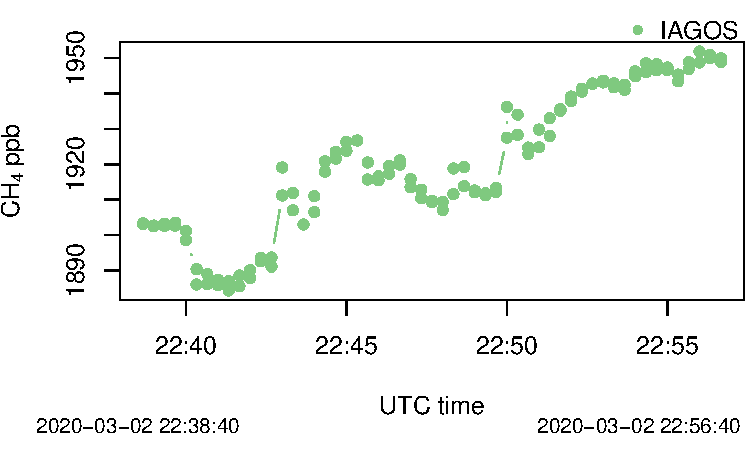
\includegraphics[keepaspectratio]{paper_files/figure-latex/unnamed-chunk-5-1.pdf}}
Finally, we show some vertical profiles for the months of January and
March of 2020. We can see how during March of 2020 methane
concentrations are lower than January. This may be due the
implementation of Lockdowns (Espinosa et al., 2023). A manuscript
focused on the impact of COVID-19 on methane emissions will be submitted
soon.

\begin{Shaded}
\begin{Highlighting}[]
\NormalTok{x }\OtherTok{\textless{}{-}}\NormalTok{ df3}
\NormalTok{x}\SpecialCharTok{$}\NormalTok{ch4 }\OtherTok{\textless{}{-}}\NormalTok{ x}\SpecialCharTok{$}\NormalTok{value}\SpecialCharTok{*}\FloatTok{1e+9}
\FunctionTok{obs\_plot}\NormalTok{(x, }
         \AttributeTok{time =} \StringTok{"ch4"}\NormalTok{, }
         \AttributeTok{y =} \StringTok{"altitude\_final"}\NormalTok{, }
         \AttributeTok{colu =} \StringTok{"month"}\NormalTok{, }
         \AttributeTok{type =} \StringTok{"b"}\NormalTok{, }
         \AttributeTok{xlab =} \FunctionTok{expression}\NormalTok{(CH[}\DecValTok{4}\NormalTok{]}\SpecialCharTok{\textasciitilde{}}\NormalTok{ppb), }
         \AttributeTok{ylab =} \StringTok{"altitude (m)"}\NormalTok{)}
\end{Highlighting}
\end{Shaded}

\begin{verbatim}
## Found the following sites: 
## [1] 1 3
## Plotting the following sites: 
## [1] 1 3
\end{verbatim}

\pandocbounded{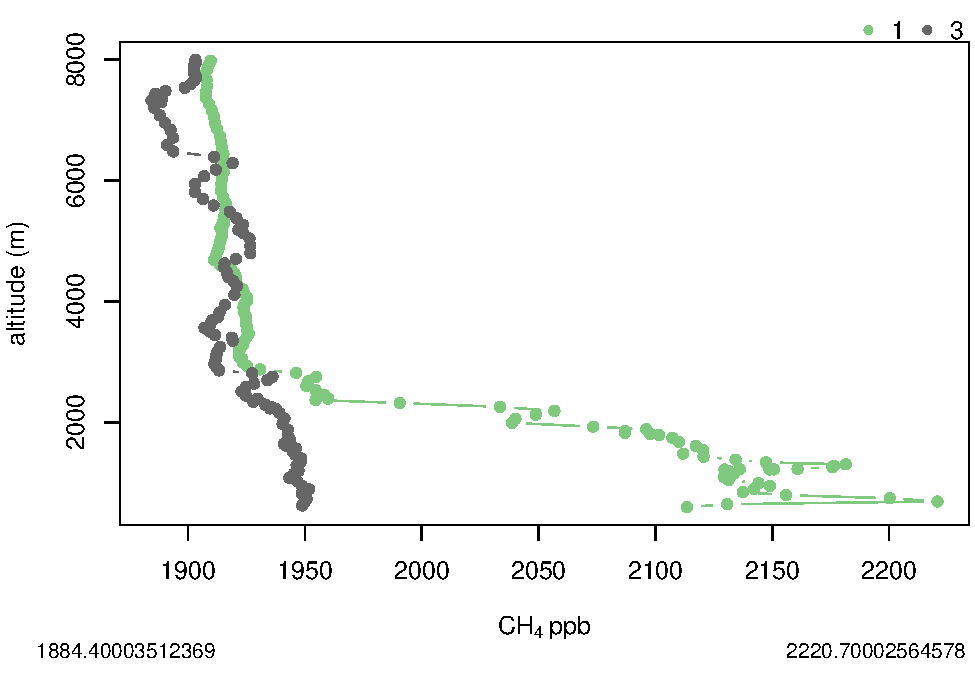
\includegraphics[keepaspectratio]{paper_files/figure-latex/unnamed-chunk-6-1.pdf}}

\subsection{Future work}\label{future-work}

We are currently porting \texttt{rtorf} to python into a package named
\texttt{pytorf} with the same functionalities. Furthermore, we expect to
implement WebAsembly with Web-R\footnote{\url{https://docs.r-wasm.org/webr/latest/}}
in R and Python to run \texttt{rtorf} on the browser (Moon, 2020).

\section{Acknowledgements}\label{acknowledgements}

This project is funded by the NOAA Climate Program Office AC4 and COM
programs (NA21OAR4310233 / NA21OAR4310234). This research was supported
by NOAA cooperative agreement NA22OAR4320151. Also, thanks to Arlyn
Andrews, John Miller, Kenneth Schuldt, Kirk Thoning and Andy Jacobson
from NOAA GML.

\section*{References}\label{references}
\addcontentsline{toc}{section}{References}

\phantomsection\label{refs}
\begin{CSLReferences}{1}{0}
\bibitem[\citeproctext]{ref-dt}
Dowle, M., \& Srinivasan, A. (2021). \emph{Data.table: Extension of
`data.frame`}. Retrieved from
\url{https://CRAN.R-project.org/package=data.table}

\bibitem[\citeproctext]{ref-espinosa2023covid}
Espinosa, S. I., Hu, L., Miller, S., Harkins, C., McDonald, B. C., Oh,
Y., Bruhwiler, L., et al. (2023). COVID-19 impacts on the US methane
emissions. \emph{AGU23}.

\bibitem[\citeproctext]{ref-lu}
Grolemund, G., \& Wickham, H. (2011). Dates and times made easy with
{lubridate}. \emph{Journal of Statistical Software}, \emph{40}(3),
1--25. Retrieved from \url{https://www.jstatsoft.org/v40/i03/}

\bibitem[\citeproctext]{ref-hunter2021glasgow}
Hunter, D. B., Salzman, J. E., \& Zaelke, D. (2021). Glasgow climate
summit: Cop26. \emph{UCLA School of Law, Public Law Research Paper},
(22-02).

\bibitem[\citeproctext]{ref-cpt}
Ibarra-Espinosa, S. (2017). \emph{Cptcity: Incorporating the cpt-city
archive into r}. Retrieved from
\url{https://CRAN.R-project.org/package=cptcity}

\bibitem[\citeproctext]{ref-lu2022methane}
Lu, X., Jacob, D. J., Wang, H., Maasakkers, J. D., Zhang, Y., Scarpelli,
T. R., Shen, L., et al. (2022). Methane emissions in the united states,
canada, and mexico: Evaluation of national methane emission inventories
and 2010--2017 sectoral trends by inverse analysis of in situ
(GLOBALVIEWplus CH\textless{} sub\textgreater{}
4\textless/sub\textgreater{} ObsPack) and satellite (GOSAT) atmospheric
observations. \emph{Atmospheric Chemistry and Physics}, \emph{22}(1),
395--418.

\bibitem[\citeproctext]{ref-lu2021global}
Lu, X., Jacob, D. J., Zhang, Y., Maasakkers, J. D., Sulprizio, M. P.,
Shen, L., Qu, Z., et al. (2021). Global methane budget and trend,
2010--2017: Complementarity of inverse analyses using in situ
(GLOBALVIEWplus CH\textless{} sub\textgreater{}
4\textless/sub\textgreater{} ObsPack) and satellite (GOSAT)
observations. \emph{Atmospheric Chemistry and Physics}, \emph{21}(6),
4637--4657.

\bibitem[\citeproctext]{ref-masarie2014obspack}
Masarie, K., Peters, W., Jacobson, A., \& Tans, P. (2014). ObsPack: A
framework for the preparation, delivery, and attribution of atmospheric
greenhouse gas measurements. \emph{Earth System Science Data},
\emph{6}(2), 375--384.

\bibitem[\citeproctext]{ref-webr}
Moon, K.-W. (2020). \emph{Webr: Data and functions for web-based
analysis}. Retrieved from \url{https://CRAN.R-project.org/package=webr}

\bibitem[\citeproctext]{ref-aggi}
NOAA GML. (2023). THE NOAA ANNUAL GREENHOUSE GAS INDEX (AGGI).
\emph{NOAA}. GML. Retrieved from
\url{https://gml.noaa.gov/aggi/aggi.html}

\bibitem[\citeproctext]{ref-R}
R Core Team. (2024). \emph{R: A language and environment for statistical
computing}. Vienna, Austria: R Foundation for Statistical Computing.
Retrieved from \url{https://www.R-project.org/}

\bibitem[\citeproctext]{ref-us2018}
Reidmiller, D. R., Avery, C. W., Easterling, D. R., Kunkel, K. E.,
Lewis, K. L., Maycock, T. K., \& Stewart, B. C. (2018). Impacts, risks,
and adaptation in the united states: Fourth national climate assessment,
volume II. doi:\href{https://doi.org/doi:\%2010.7930/NCA4.2018}{doi:
10.7930/NCA4.2018}

\bibitem[\citeproctext]{ref-rhodes20162015}
Rhodes, C. J. (2016). The 2015 paris climate change conference: COP21.
\emph{Science progress}, \emph{99}(1), 97--104.

\bibitem[\citeproctext]{ref-saunois2016global}
Saunois, M., Bousquet, P., Poulter, B., Peregon, A., Ciais, P.,
Canadell, J. G., Dlugokencky, E. J., et al. (2016). The global methane
budget 2000--2012. \emph{Earth System Science Data}, \emph{8}(2),
697--751.

\bibitem[\citeproctext]{ref-saunois2020global}
Saunois, M., Stavert, A. R., Poulter, B., Bousquet, P., Canadell, J. G.,
Jackson, R. B., Raymond, P. A., et al. (2020). The global methane budget
2000--2017. \emph{Earth system science data}, \emph{12}(3), 1561--1623.

\bibitem[\citeproctext]{ref-epagwp}
S.EPA, U. (2023). Understanding global warming potentials. \emph{EPA}.
Environmental Protection Agency. Retrieved from
\url{https://www.epa.gov/ghgemissions/understanding-global-warming-potentials\#:~:text=Methane\%20(CH4)\%20is\%20estimated,more\%20energy\%20than\%20CO2.}

\bibitem[\citeproctext]{ref-Silge2016}
Silge, J., \& Robinson, D. (2016). Tidytext: Text mining and analysis
using tidy data principles in r. \emph{Journal of Open Source Software},
\emph{1}(3), 37.
doi:\href{https://doi.org/10.21105/joss.00037}{10.21105/joss.00037}

\bibitem[\citeproctext]{ref-wh}
U.S. White House. (2021, September). Joint US-EU press release on the
global methane pledge. \emph{The White House}. The United States
Government. Retrieved from
\url{https://www.whitehouse.gov/briefing-room/statements-releases/2021/09/18/joint-us-eu-press-release-on-the-global-methane-pledge/}

\end{CSLReferences}

\end{document}
